\section{Bulk density, spatial structure, and finite-size lifetimes}
\label{sec:sbulk}

The extended campaign resolves finite bulk activity close to front
reversal on large systems and long observation windows (Fig.~\ref{fig:gpu_bulk}). At $q=0.04594$, all four $L=8192$
random-start runs remain active through $5\times10^6$ steps. Their
unconditional mean density over $2.5$--$5\times10^6$ is $0.28659$, with a
pointwise 95\% run-bootstrap interval $[0.28651,0.28667]$.
The difference between the second and first halves of this late window is
$7.2\times10^{-5}$, with interval $[-8.7\times10^{-5},1.6\times10^{-4}]$.
Thus no systematic late-window density decrease is resolved at this sampled
point; the spatial and front checks test its relation to coexistence separately.
Doubling the size to $L=16384$ gives a mean of 0.28661 at the same $q$
and time window. All twelve $L=16384$ runs at $q=0.04592$, 0.04594,
and 0.04596 remain active through $5\times10^6$ steps; none of the
three cohorts resolves a late-window density drift. The corresponding
means are 0.28498, 0.28661, and 0.28803. This comparison extends the
finite-density branch to substantially larger systems near front reversal.
At $q=0.04594$, the matched $2$--$5\times10^6$ window gives
$\chi_{8192}/\chi_{4096}=0.97$ with a pointwise 95\% run-bootstrap
interval $[0.84,1.08]$. The four independent runs at each size show no resolved
increase of this magnetic fluctuation scale upon doubling $L$.
The further doubling gives $\chi_{16384}/\chi_{8192}=0.95$ with interval
$[0.78,1.14]$ over the same window, again with no absorption in either
four-run cohort.

\begin{figure*}
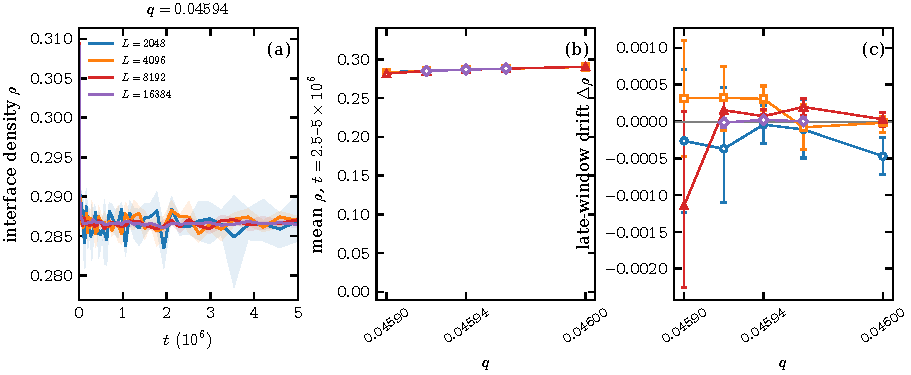
\includegraphics[width=\textwidth]{figs/fig_gpu_bulk}
\caption{Long, large-system bulk tests at $p=\alpha=1/2$, with four independent
random starts per $(L,q)$ and $T=5\times10^6$.
(a) Interface density at $q=0.04594$; bands are pointwise 95\% run-bootstrap
intervals. (b) Unconditional time-weighted density over
$2.5\times10^6\le t\le5\times10^6$ against the actual probability $q$.
(c) Difference between means over $3.75$--$5\times10^6$ and
$2.5$--$3.75\times10^6$; zero indicates no resolved drift between these
windows. Error bars in (b,c) are 95\% run-bootstrap intervals.
Every declared seed contributes; absorbed trajectories contribute their known
absorbing state for the rest of the observation window.}
\label{fig:gpu_bulk}
\end{figure*}

The final configurations provide a direct spatial check
(Fig.~\ref{fig:spatial_v2}). At $q=0.04594$, both $L=8192$ and 16384
give $C(128)\simeq0.0046$. For $L=16384$, $C(r)$ decreases from
0.427 at one lattice spacing to $5.7\times10^{-4}$ at $r=256$;
the pointwise intervals at $r=512$ and 1024 include zero. Signed
long-distance fluctuations are retained rather than clipped or fitted
to an assumed positive tail. The observed decay occurs on scales much
smaller than the box, complementing the density and magnetic-moment
comparisons. These are final-time measurements, not an extrapolation
of a correlation length to the transition.

\begin{figure*}
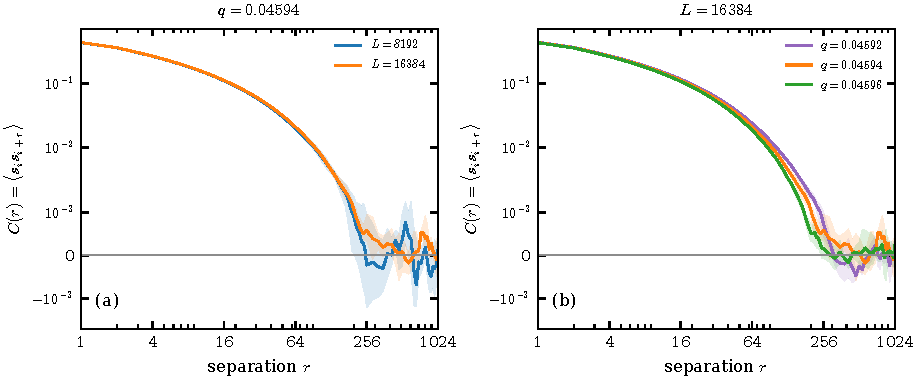
\includegraphics[width=\textwidth]{figs/fig_spatial_v2}
\caption{Direct spatial correlations at $p=\alpha=1/2$, measured in the
final configurations at $T=5\times10^6$, with four independent runs per
curve. The observable is the raw axis-averaged spin product in
Eq.~\eqref{M-eq:correlation}. (a) Size comparison at $q=0.04594$.
(b) Three probabilities at $L=16384$. Shading gives pointwise 95\%
run-bootstrap intervals; all declared configurations are included.
The vertical scale is logarithmic outside $|C|\le10^{-3}$ and linear
inside that interval, displaying both signs of the small long-distance
fluctuations. No functional form is fitted.}
\label{fig:spatial_v2}
\end{figure*}

Earlier bulk runs from random initial conditions (Fig.~\ref{fig:bulk}) give late-window
estimates of the active-phase interface density. At the points above $\qs$
shown in this survey, it settles within $10^3$--$10^4$ steps and then stays
constant to the end of the runs ($t = 2\times10^5$--$10^6$), independently of $L$ from 256 to 4096
within the run-to-run errors: $\rho = 0.3021$--$0.3023$ at $q = 0.046359$
and $0.3108$--$0.3113$ at $q=0.046818$
[Fig.~\ref{fig:bulk}(b)]. Even at $q = 0.0459$, the active phase
holds $\rho\simeq0.28$ for the full run ($10^6$ steps for $L\le 1024$, $3\times10^5$ and
$2\times10^5$ for $L = 2048$ and 4096) at every $L\ge 512$.
Such persistence can occur on the metastable side, so bulk persistence alone
does not locate the boundary. The finite-density branch persists to the
front-reversal region, supporting a discontinuity of order 0.28.
The magnetic second moment of the active phase,
$\chi_L = L^2\langle m^2\rangle$, grows toward the transition: its estimates are
$60$--$66$ at $q=0.05049$ and $305$--$463$ at $q=0.046359$ for $L=512$--4096.
At $q=0.0459$ they are of order $10^3$ for $L\ge1024$, with substantial
run-to-run uncertainty and no resolved growth with size. These data constrain magnetic fluctuations
at the sampled active points, rather than excluding an unsampled critical interval.
Measured directly from stored configurations at $q=0.046359$ ($L = 2048$,
$t\ge 10^5$), the two-point function of the local spin $s_i=2\sigma_i-1$
falls to $0.40$ at one lattice spacing. Local exponential fits give
$\xi = 15$--$18$ over $4\le r\le 40$ and $10\le r\le 60$; at $q=0.05049$,
$\xi = 7$--$9$.

On the sampled lower-$q$ side, the active phase exhibits metastable decay. At $q = 0.045441$ its density stays within 12\% of
the apparent active-branch plateau for $10^4$ steps and then collapses at an accelerating rate
[Fig.~\ref{fig:bulk}(a)]. The accelerating collapse and visible growth of absorbing
droplets [Fig.~\ref{M-fig:snap}(b)] support nucleation-driven decay.
Where droplets of opposite type meet, a layer of the active phase
remains between them (Sec.~\ref{M-sec:wall}), so $\rho$ does not drop to zero at once but to a slowly
coarsening network of wetted walls. The recorded half-density time $\tau$ grows steeply as
$q\to\qs$: $\tau = 3.4\times10^3$, $8.0\times10^3$, $1.6\times10^4$, $2.6\times10^4$, and
$7.0\times10^4$ at $q=0.04131$, 0.043605, 0.044523, 0.044982, and 0.045441.
It saturates at large $L$ [Fig.~\ref{fig:bulk}(c)]; at the closest of these points,
the means are $7.33$, $7.04$, $6.65$, and $6.70\times10^4$ for
$L=512$, 1024, 2048, and 4096. Many droplets nucleate independently, and the decay is a local
process (the multi-droplet regime of Ref.~\cite{rikvold1994}). Smaller systems ($L\le 128$) decay
sooner, because their size is only a few correlation lengths of the active phase, so that
the whole lattice can reach an absorbing state through one fluctuation.

\begin{figure*}
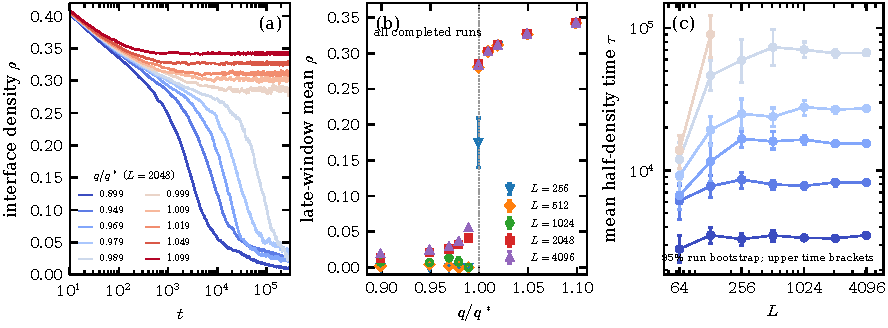
\includegraphics[width=\textwidth]{figs/fig_bulk05}
\caption{Bulk runs at $p = 1/2$ from random initial conditions ($\qs = 0.04594$). (a) Interface
density against time at $L = 2048$ for $q/\qs$ from 0.9 to 1.1 (one seed each).
(b) Time-weighted late-window density against $q/\qs$ for $L = 256$--4096,
using every completed run and all records over $t\ge T/2$ (2--16 runs per point).
Absorbed trajectories contribute zero after absorption; no activity filter is applied.
(c) Mean recorded half-density time below $\qs$ against $L$, shown only for
groups in which every trajectory crossed the threshold by the final time.
Times are first recorded crossings, including $10^3$ for five left-censored
$L=64$ runs; bars are 95\% run-bootstrap intervals, separate from output-cadence effects
(32 runs for $L\le
128$, 2--16 above; $T = 10^6$ for $L\le 1024$, $3\times10^5$ and $2\times10^5$ for $L = 2048$ and
4096).}
\label{fig:bulk}
\end{figure*}

The size dependence above $\qs$ is the opposite. Earlier $10^6$-step
cohorts at $q=0.046359$ had 32 of 32 consensus events at $L=64$, 25 of 32
at $L=128$, and none of 16 at $L=256$. We now test this stability signature
with independent, longer cohorts, keeping the two data sets separate.

A separate fixed ensemble extends the finite-size comparison at
$p=\alpha=1/2$, $q=0.046359$ to $T=10^7$ steps, with 32 independent
random starts at each of $L=64$, 128, 192, and 256
(Fig.~\ref{fig:lifetimes_v2}). The numbers reaching consensus are
32, 32, 6, and 0, respectively. The first recorded crossings of
$\rho<0.145$ are more frequent: 32, 32, 16, and 1.
Thus loss of half the reference activity and complete absorption are
separate observables. At $L=256$, the unconditional mean density over
$5\times10^6\le t\le10^7$ is 0.30230, with a 95\% run-bootstrap
interval $[0.30213,0.30246]$. With no consensus event among 32 $L=256$ runs,
the exact two-sided 95\% lower confidence limit for survival through
$10^7$ steps is 0.891. These observations extend the persistence window
and resolve strong size dependence; they do not determine an
asymptotic lifetime law.

The same contrast persists closer to coexistence. At $q=0.04605$, a
separate fixed ensemble follows 16 random starts at each of $L=192$,
256, and 384 to $3\times10^6$ steps. Consensus counts are 15, 6, and 0,
while recorded half-density events number 16, 6, and 1. The unconditional
mean densities over $1.5$--$3\times10^6$ are 0.060, 0.199, and 0.29235,
respectively. At $L=384$, the 95\% run-bootstrap density interval is
$[0.29100,0.29325]$,
and the exact two-sided 95\% lower confidence limit for survival through
the horizon is 0.794. Thus the size-dependent stability signature is
present at a second probability closer to the front-reversal region.

\begin{figure*}
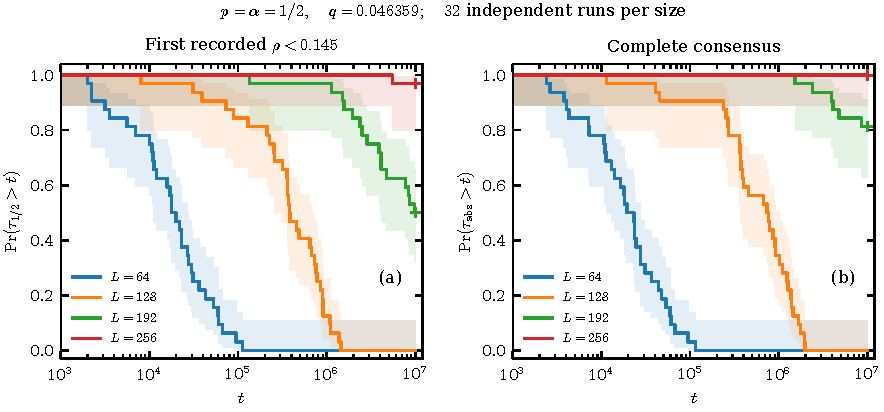
\includegraphics[width=\textwidth]{figs/fig_lifetimes_v2}
\caption{Long finite-size trajectories at $p=\alpha=1/2$, $q=0.046359$:
32 independent random starts per size, all followed until consensus or
$T=10^7$ steps. (a) Survival of the first recorded $\rho<0.145$ event,
searched at $t\ge10^3$ on the regular 1000-step and additional logarithmic
observation grid; recording-grid limitations are discussed in
Sec.~\ref{M-sec:methods}. (b) Survival to complete consensus.
Event counts for $L=64,128,192,256$ are $(32,32,16,1)$ in (a) and
$(32,32,6,0)$ in (b). Crosses denote right censoring. Shading gives
pointwise 95\% Kaplan--Meier bands (Greenwood log--log intervals away
from zero and one, with exact binomial edge bounds).}
\label{fig:lifetimes_v2}
\end{figure*}

In a multi-droplet description, the half-density time scales as
$\tau\propto(Iv^2)^{-1/3}$, where $I$ is the nucleation rate per unit area and
$v$ is the growth speed~\cite{rikvold1994}. The steep increase of $\tau$ on
approaching coexistence is consistent with slowing fronts and rarer nucleation.
Our finite interval of control parameters does not determine an asymptotic
nucleation law. In particular, a fit over these points cannot establish or
exclude the essential singularity expected from a classical nucleation barrier.

